\chapter{Designing the Data-Collection FSM \\(A dataset we can trust)}
\label{ch:data-collection}

\section{Why a data-collection FSM at all?}
Chapter~\ref{ch:fsm-basics} argued that finite state machines give us clarity, testability, and instrumentation—
especially the power to log clean datasets from a process that involves randomness. \cite{fsm_superpowers}
Instrumenting a randomized process is the heart of empirical simulation:
if we cannot exactly say when and what we recorded, we cannot trust the results.

This chapter produces two practical deliverables:

\begin{enumerate}
  \item A precise list of \textbf{fields} that define one Monty Hall trial (one row in a CSV).
  \item A clear \textbf{Data-Collection FSM} that spells out what happens, when it happens, what we log, and when we stop.
\end{enumerate}

\section{The per-trial log (one row per game)}
We record one row per simulated trial. These fields are the minimum needed to:
verify randomness, debug mistakes, and compute meaningful statistics.

\begin{table}[!ht]
\centering
\caption{Trial log fields (one row per simulated game).}
\label{tab:trial-fields}
\begin{tabular}{ll}
\toprule
Field & Meaning and reason to include \\
\midrule
trial\_id & Unique integer for traceability and reproducibility \\
seed & RNG seed (optional) to reproduce a suspicious run \\
prize\_door & Where the prize was placed (should be uniform over \{1,2,3\}) \\
player\_door & Player’s initial choice (should be uniform over \{1,2,3\}) \\
reveal\_door & Host’s revealed goat door (≠ prize\_door, ≠ player\_door) \\
decision & \texttt{stay} or \texttt{switch} (coin toss in baseline) \\
final\_door & Door the player ends on after decision \\
win & \texttt{1} if final\_door == prize\_door, else \texttt{0} \\
strategy & \texttt{random}, \texttt{always\_stay}, \texttt{always\_switch} (for experiments) \\
\bottomrule
\end{tabular}
\end{table}

Each field serves a purpose:
\begin{itemize}
  \item \textbf{trial\_id} and \textbf{seed} let us exactly reproduce a particular run later.
  \item \textbf{prize\_door, player\_door, reveal\_door} capture the full story of a single game.
  \item \textbf{decision, final\_door, win, strategy} are the core outcomes we analyze.
\end{itemize}

\section{What we aggregate as we go (running totals)}
Along with the detailed per-trial row, we maintain running counters for three reasons:

\begin{enumerate}
  \item Display progress without rereading the entire log.
  \item Build plots efficiently from incremental values.
  \item Decide when we have enough trials to make trustworthy claims.
\end{enumerate}

At minimum, track these four outcome buckets:
\begin{itemize}
  \item \texttt{stay\_win}
  \item \texttt{stay\_lose}
  \item \texttt{switch\_win}
  \item \texttt{switch\_lose}
\end{itemize}

Add distribution checks to catch mistakes or bias:
\begin{itemize}
  \item Counts of \texttt{prize\_door} = 1,2,3
  \item Counts of \texttt{player\_door} = 1,2,3
  \item Counts of \texttt{decision} stay vs switch
\end{itemize}

These sanity checks show immediately if something like door 3 never gets chosen or
if randomness is skewed.

\section{When do we stop? \\Confidence, not vibes}
We want students to understand the difference between:
\begin{quote}
\emph{We ran a bunch of trials.} \quad vs \quad \emph{We ran enough trials to support a claim.}
\end{quote}

To decide when to stop, we base the rule on a confidence interval for a proportion
(the win rate).  
Let $\hat{p}$ be the observed win rate for a strategy after $n$ trials.
A widely used approximate margin of error, often called the halfwidth of a confidence
interval, is:

\[
  \mathrm{halfwidth} = z \sqrt{\frac{\hat{p}(1-\hat{p})}{n}}
\]

Here:
\begin{itemize}
  \item $\hat{p}$ is the observed win rate.
  \item $n$ is the number of trials for that strategy.
  \item $z$ is the z-score that matches the chosen confidence level:
    \begin{itemize}
      \item about $1.645$ for 90\% confidence,
      \item about $1.96$ for 95\%,
      \item about $2.576$ for 99\%.
    \end{itemize}
\end{itemize}

This is the normal‑approximation form for a proportion confidence interval; it is
simple, intuitive, and commonly used for large enough samples. NIST documents this
normal approximation among its supported methods for computing proportion confidence
limits. :contentReference[oaicite:1]{index=1}

\subsection{A practical stopping rule}
Choose two things up front:
\begin{itemize}
  \item A confidence level: 90\%, 95\%, or 99\%.
  \item A tolerance $\epsilon$: how large a halfwidth you are willing to accept.
        Example: $\epsilon = 0.01$ means you want the halfwidth to be at most
        $\pm 1\%$ around the observed win rate.
\end{itemize}

Stop the simulation only when \textbf{both} strategies’ win‑rate halfwidths are
no larger than $\epsilon$:

\begin{itemize}
  \item halfwidth of switch win‑rate $\le \epsilon$
  \item halfwidth of stay win‑rate   $\le \epsilon$
\end{itemize}

This makes the simulation self‑aware: it continues until the estimates are sharp
enough to be worth graphing or reporting.

\subsection{Why this stopping rule matters}
\begin{itemize}
  \item If you stop too early, your estimates are noisy; the interval is wide.
  \item If you require very high confidence or very small tolerance, you may need
    many trials.
  \item The rule explicitly ties the stopping decision to the precision of the
    estimate, not to an arbitrary trial count or a whim.
\end{itemize}

\section{Worst-case estimate of needed trials}
Because $\hat{p}(1-\hat{p})$ is largest when $\hat{p}=0.5$, we can derive a
conservative bound on how many trials might be necessary.

\[
 n \ge \frac{z^2}{4\epsilon^2}
\]

Derivation sketch:
\begin{itemize}
  \item Replace $\hat{p}(1-\hat{p})$ by its maximum value $1/4$.
  \item Solve the inequality $z \sqrt{\frac{1/4}{n}} \le \epsilon$ for $n$.
\end{itemize}

Example: for 99\% confidence ($z \approx 2.576$) and $\epsilon = 0.01$,

\[
 n \gtrsim \frac{(2.576)^2}{4(0.01)^2} \approx 16588.
\]

This number is intentionally large to demonstrate why a few hundred trials can still
be noisy for tight tolerances. It is a worst‑case estimate; actual needed $n$ could
be smaller if the observed $\hat{p}$ is far from $0.5$, but it gives students a
sense of scale.

\section{The data‑collection FSM (EFSM style)}
When we track extra variables such as \texttt{prize\_door} and \texttt{player\_choice},
we’re really building an \emph{extended} FSM, or EFSM. Our Data-Collection FSM uses
the same clean state backbone as in Chapter~\ref{ch:fsm-basics}, but now annotates
each step with:
\begin{itemize}
  \item Which variables are set at that step.
  \item What gets logged.
  \item What gets aggregated.
  \item When the stopping rule is evaluated.
\end{itemize}

\begin{figure}[!ht]
  \centering
  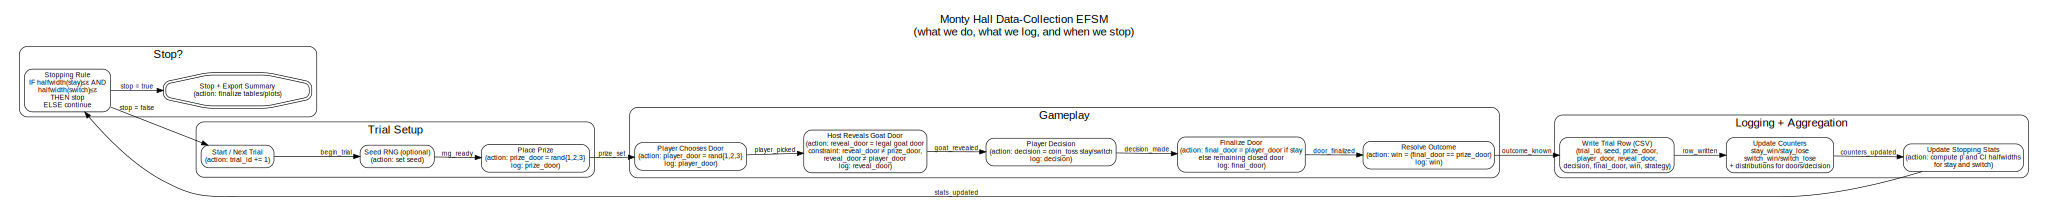
\includegraphics[width=\linewidth]{data_collection_fsm.pdf}
  \caption{Data-Collection FSM for Monty Hall simulation (Graphviz-generated).}
  \label{fig:data-collection-fsm}
\end{figure}

\section{How this maps to code (preview of Chapter 4)}
The FSM‑to‑code recipe from Chapter~\ref{ch:fsm-basics} still applies:
\begin{itemize}
  \item State enumeration,
  \item Events,
  \item Transition function,
  \item Actions on transitions.
\end{itemize}

The new difference is that actions include:
\begin{itemize}
  \item Writing a trial row to CSV,
  \item Updating running counters,
  \item Computing confidence halfwidths and checking whether to stop.
\end{itemize}

Designing this chapter first makes the FSM the contract for the implementation
and for unit tests, ensuring both correctness and clarity.
